\section{Facebook}
\label{sec:facebook}

%------------------------------------------------------------------------

\begin{figure}[!h]
\centering
\begin{subfigure}{.5\textwidth}
  \centering
  
\includegraphics[width=.4\linewidth]{images/lukasz/pobrane.jpg}
  \caption{Logo graficzne}
  \label{fig:sub1}
\end{subfigure}%
\begin{subfigure}{.5\textwidth}
  \centering
  
\includegraphics[width=.4\linewidth]{images/lukasz/facebook-logo.jpg}
  \caption{Logo tekstowe}
  \label{fig:sub2}
\end{subfigure}
\captionsource{Logo portalu społecznościowego Facebook'a}{\url{http://facebook.com/}}
\label{fig:logo-facebook}
\end{figure}


Facebook --- jako termin encyklopedyczny to serwis społecznościowy, w ramach którego zarejestrowani użytkownicy mogą tworzyć sieci i grupy, dzielić się wiadomościami i zdjęciami oraz korzystać z aplikacji, będących własnością Facebook, Inc. z siedzibą w Menlo Park. W styczniu 2014 liczba użytkowników na całym świecie wynosiła około miliarda, a co miesiąc wgrywanych jest ponad 1 mld zdjęć oraz 10 mln filmów, których obecnie jest 265 miliardów. Średni wiek użytkownika serwisu to 22 lata. Dane zgromadzone na Facebooku to ponad 180 petabajtów, co 24 godziny przybywa ponad 0,5 petabajta.

%------------------------------------------

\subsection{Historia}
Serwis stworzył Mark Zuckerberg wraz z grupą swych przyjaciół jeszcze jako student Uniwersytetu Harvarda. Na początku był to on-line The Facebook, Serwis ten umożliwiał zarejestrowanym użytkownikom odszukanie i kontynuację szkolnych znajomości, a także pozwalał na dzielenie się wiadomościami oraz zdjęciami. Zuckerbergowi stworzenie kodu źródłowego zajęło dwa tygodnie. Serwis od chwili uruchomienia bardzo szybko zyskał zainteresowanie studentów uczelni, na której powstał. Liczba studentów, która zarejestrowała się na nowej stronie w przeciągu dwóch tygodni od jej powstania  przekroczyła 2/3 wszystkich studentów Harvarda.

Na fali popularności młody twórca decyduje się na poszerzenie zasięgu swojej strony o inne szkoły. Kolejnym krokiem jest więc zawiązanie współpracy ze swym współlokatorem Dustinem Moskovitzem. Uniwersytet Stanforda, Columbia, oraz Yale to kolejne uczelnie, które zostały objęte zasięgiem serwisu \cite{url:wiki-facebook}.

%------------------------------------------

\subsection{Facebook w Polsce}
\label{subsec:facebook-w-polsce}
W maju 2008 roku rusza polska wersja językowa serwisu. Dzisiaj Facebook to najpopularniejszy serwis społecznościowy w Polsce, który liczy 15 mln zarejestrowanych użytkowników. Z Facebooka korzysta 27,73\% mieszkańców i 44,76\% internautów z Polski. Najwięcej członków portalu z naszego kraju ma od 18 do 24 lat (3,2 mln), a następne grupy wiekowe to 25-34, 35-44, 13-15 i 16-17. 52\% użytkowników Facebooka z Polski stanowią kobiety, 48\% to mężczyźni \cite{url:wp-facebook-w-polsce}.

%------------------------------------------

\subsection{Możliwości promocji}
Facebook daje firmom, a także korporacjom, bardzo szerokie możliwości w dziedzinie marketingu. Z początku serwis kierowany był do osób indywidualnych, a firmy zakładały swe konta jako osoby prywatne. Przyjmowały do swojego grona znajomych  i funkcjonowały jak zwykli pojedynczy użytkownicy. 

%------------------------------------------

\subsubsection{Fanpage}
Z biegiem czasu liczba firm posiadających swe konta w serwisie, wzrosła do takiej liczby, iż twórcy facebooka postanowili stworzyć specjalny rodzaj kont dedykowany pod firmy, korporacje oraz organizacje. Były to strony fanpage'owskie czyli fanpage'e widoczne na rysunku \ref{fig:facebook-fanpage}. Posiadają one różne funkcje, zależne od specyfiki firmy i jej potrzeb.

\begin{figure}[!ht]
\centering
    \scalebox{0.4}
    {
        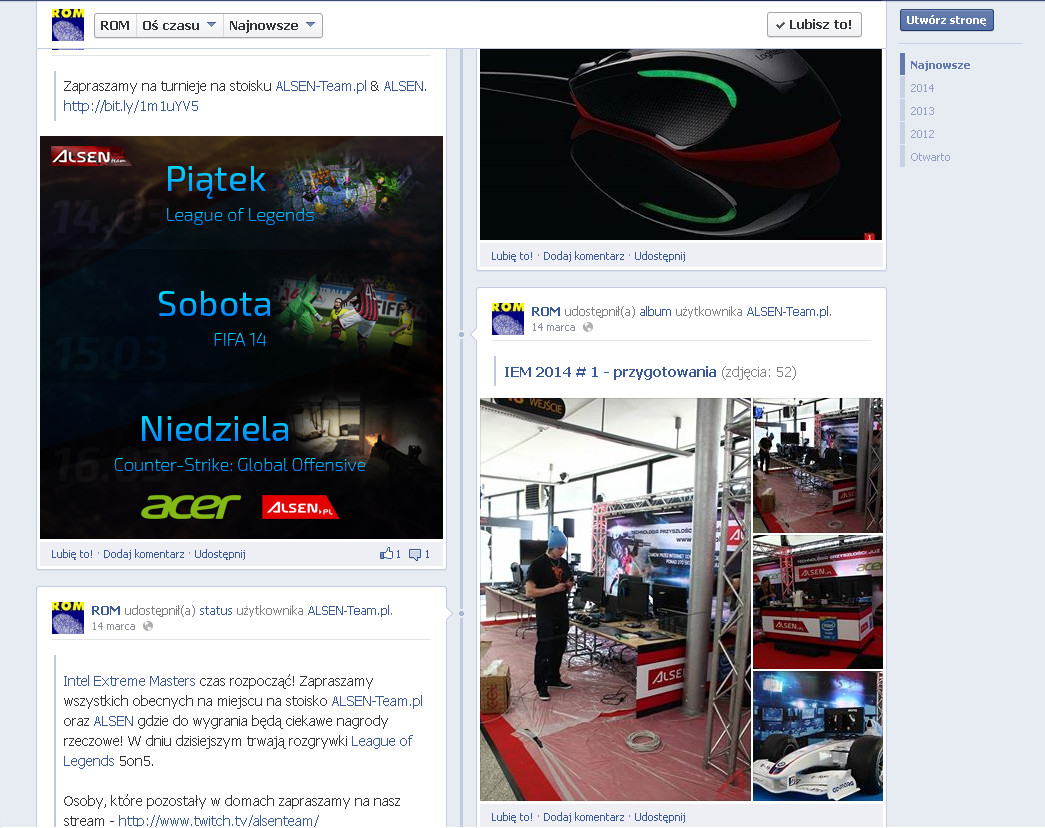
\includegraphics{images/lukasz/fan.png}
    }
    \captionsource{Fanpage sklepu komputerowego na serwisie Facebook}{Opracowanie własne na podstawie: \url{https://www.facebook.com/pages/ROM/107709282653888?fref=ts}}
    \label{fig:facebook-fanpage}
\end{figure}

W przeciwieństwie do osób prywatnych, fanpage'e nie mają możliwości dodawania znajomych, a co za tym idzie ich posiadania. Mają fanów, u których pojawiają się na tablicach informacje --- posty zamieszczane przez firmę. Facebook umożliwia także firmom, poza posiadaną przez nie (firmy) funkcją publikowania wiadomości w formie tekstowej, zdjęć, plików audio i wideo, także funkcją służącą zamieszczaniu linków do treści zewnętrznych poza zamieszczonych poza fanpagem danej firmy na jej profilu facebookowym, dostęp do szerokiej gamy aplikacji, które mają na celu wspomagania interakcji z użytkownikami. Firma może tworzyć wydarzenie, na które chce zaprosić swych fanów --- tym samy promując swe przedsięwzięcie, a także zadawać pytania i dzięki temu poznawać opinie swych fanów na różne tematy.


\subsubsection{Aplikacje}
Firmy i korporację, które są w sposób bardziej zaawansowany zaznajomione z działanie portali społecznościowych i ich możliwościami facebook oferuje zaimplementowanie na swoim fanpage'u aplikacji. Mogą być one w formie quizów --- konkursów, bądź też zabaw interaktywnych. Mogą być one ciekawym urozmaiceniem w nawiązywaniu kontaktów pomiędzy obecnymi, bądź przyszłymi klientami (fanami), a firmą. Może to z kolei zaowocować powiększającym się gronem osób będących na danym fanpage’u, dzięki systemowi poleceń. Wygląda to obiecująco. Wadą takiego rozwiązania jest fakt, iż napisanie takiej aplikacji należy zlecić dobremu programiście, który zadba o właściwe funkcjonowanie, jak również stabilne działanie danej aplikacji, co przekłada się na dodatkowy koszt związany z chęcią zaistnienia w mediach społecznościowych.


\subsubsection{Statystyka}
Ta funkcja jest dostępna dla administratorów firmowych stron fanowskich na facebooku --- ,,usługa statystyki pozwala na usprawnienie zbierania i analizowania danych o stronach fanowskich'' \cite{url:hatalska-mikroblogi}. Można tam znaleźć informacje dotyczące aktywności fanów na danej stronie, liczbie osób ją odwiedzających ilości kliknięć ,,lubię to'' pod każdym z postów zamieszczonych pod każdym z opublikowanego postu, liczbie komentarzy pod danym wpisem, dane o tym ile razy fani wchodzą w danym okresie czasu na poszczególne podstrony danej strony (np. tablica, zdjęcia). Zamieszczone są tam także informacje jak dane demograficzne fanów danej strony jak płeć, wiek, kraj zamieszkania, miasto, a także język jakim się posługują. Tego typu dane są dostępne dla administratorów fanpage'ów, posiadających uprawnienia od firmy, którą reprezentują do wszelkich dostępnych działań na stronie fanowskiej, takich jak: publikowanie oraz przeglądania statystyk.

\begin{figure}[!h]
\centering
    \scalebox{0.41}
    {
        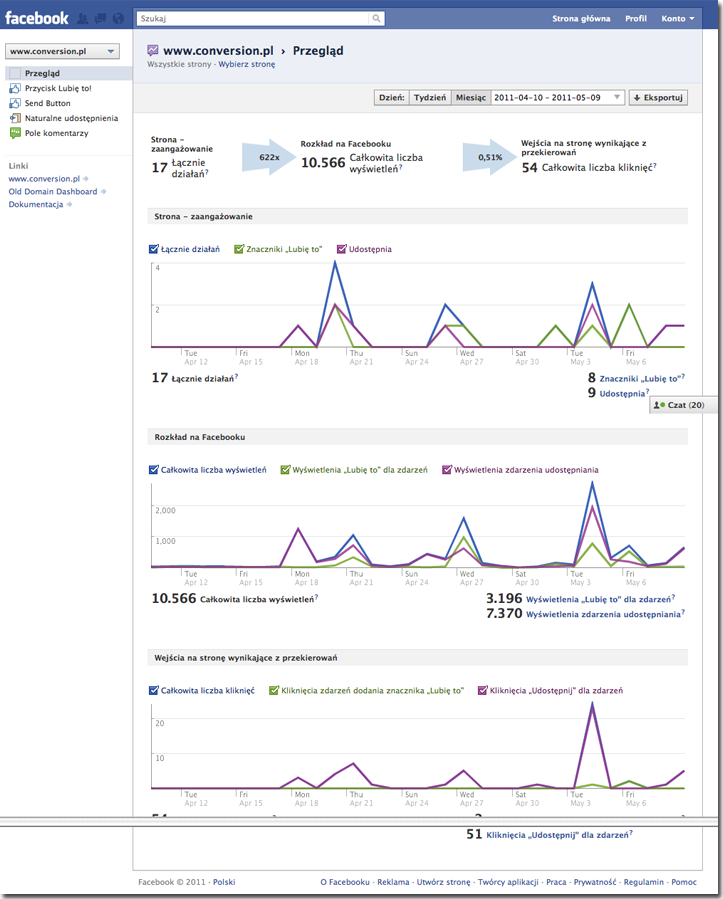
\includegraphics{images/lukasz/dashboard-facebook.png}
    }
    \captionsource{Wykres statystyk facebook’a}{Opracowanie własne na podstawie \cite{url:facebook-sledzenie-klinkiec}}
    \label{fig:facebook-stat-page}
\end{figure}

Z poniższego rysunku \ref{fig:facebook-stat-page} jasno wynika, iż statystyki są dostępne jako czytelny i przystępny wykres, który jest pomocny przy ocenie popularności danego fanpage’a, pozwalają wymusić na jej twórcach działania, które spełnią oczekiwania odbiorców --- ,,te wskaźniki są doskonałym materiałem do analizy efektywności strony fanowskiej, gdyż możesz dzięki nim dowiedzieć się kim są Twoi fani, gdzie mieszkają, jakie grupy wiekowe reprezentują i jakimi językami się posługują'' \cite{url:darmowe-piwo-przez-facebook}.\\

\hfill Autor: \textit{Łukasz Suder}